\section{Gauss elimination for dense matrix}
\subsection{Solution for triangular systems}
\begin{alg}
    \label{alg::back-substitution}
    To solve the triangular systems of equations 
    $\mathbf{Ux=c}$, where $\mathbf{U}$ is upper
    triangular, we use back-substitution as follows.
    \IncMargin{1em}
    %\LinesNumbered
    \begin{algorithm}[H]
        \caption{Back-substitution}
        \SetKwInOut{Precond}{Preconditions}
        \SetKwInOut{Postcond}{Postconditions}

        \KwIn{$\mU\in\mathbb{R}^{n\times n},\,\mathbf{c}
        \in\mathbb{R}^n$}
        \Precond{$\mU$ is upper triangular, $u_{kk}\neq 0,\,
        k=1,2,\ldots,n$}
        \KwOut{The solution $\mx$ of $\mU\mx=\mathbf{c}$}

        \BlankLine
        $x_n=c_n/u_{nn}$\;
        \For{$k=n-1,n-2,\ldots,1$}{
        $x_k=\left(c_k-\sum_{j=k+1}^n u_{kj}x_j\right)/u_{kk}$\;
        }
    \end{algorithm}
    \DecMargin{1em}
\end{alg}

\begin{alg}
    \label{alg::back-substitution}
    To solve the triangular systems of equations 
    $\mathbf{Lx=b}$, where $\mathbf{L}$ is lower
    triangular, we use forward substitution as 
    follows.
    \IncMargin{1em}
    %\LinesNumbered
    \begin{algorithm}[H]
        \caption{Forward substitution}
        \SetKwInOut{Precond}{Preconditions}
        \SetKwInOut{Postcond}{Postconditions}

        \KwIn{$\mL\in\mathbb{R}^{n\times n},\,\mathbf{b}
        \in\mathbb{R}^n$}
        \Precond{$\mL$ is lower triangular, $l_{kk}\neq 0,\,
        k=1,2,\ldots,n$}
        \KwOut{The solution $\mathbf{c}$ of 
        $\mL\mathbf{c}=\mathbf{b}$}

        \BlankLine
        $c_1=b_1/l_{11}$\;
        \For{$k=2,3,\ldots,n$}{
        $c_k=\left(b_k-\sum_{j=1}^{k-1} l_{kj}c_j\right)/l_{kk}$\;
        }
    \end{algorithm}
    \DecMargin{1em}
\end{alg}

\begin{prop}
    Basic to all general-purpose direct methods for 
    solving equation $\mathbf{Ax=b}$ is the
    concept that triangular systems of equations are 
    ‘easy’ to solve.
\end{prop}

\subsection{Gaussian transform}
\begin{defn}[Gaussian transform]
    \label{defn::GaussTransform}
    For a given vector $\mathbf{x}\in\mathbb{R}^n$, define
    $$
        \mathbf{L}_k=\mathbf{I}-\mathbf{l}_k
        \mathbf{e}_k^T=
        \begin{bmatrix}
            1&\\
             &\ddots\\
             &      &1\\
             &      &-l_{k+1,k}&1\\
             &      &\vdots    &&\ddots\\
             &      &-l_{nk}  &&      &1
        \end{bmatrix},
    $$ 
    where $\mI$ is the unitary matrix, $\mathbf{l}_k=(0,\ldots,0,l_{k+1,k},\ldots,l_{nk})^T$ and $l_{ik}=x_i/x_k,
    i=k+1,\ldots,n$, 
    $\mathbf{e}_k$ has an only nonzero entry $1$ at the 
    $k$-th component. Therefore, $\mathbf{L}_k\mathbf{x}=
    (x_1,\ldots,x_k,0,\ldots0)^T$. Matrix $\mathbf{L}_k$ is
    called \it{Gaussian transform} or \textit{elementary lower 
    triangular} matrix.
\end{defn}

\begin{lem}
    \label{lem::GaussInverse}
    $\mathbf{L}_k^{-1}=\mathbf{I}+\mathbf{l}_k\mathbf{e}_k^T$.
\end{lem}
\begin{proof}
    By definitions of $\mathbf{l}_k$ and $\mathbf{e}_k$, we have
    $\mathbf{e}_k^T\mathbf{l}_k=0$, so
    $$
        (\mathbf{I}-\mathbf{l}_k\me_k^T)(\mI+\ml_k\me_k^T)=
        \mI-\ml_k\me_k^T\ml_k\me_k^T=\mI.
    $$ 
\end{proof}

\begin{lem}
    \label{lem::GaussIverseMulti}
    $$
    \mL_1^{-1}\ldots\mL_{n-1}^{-1}=
    \begin{bmatrix}
        1\\
        l_{21}&1\\
        \vdots&\vdots&\ddots\\
        l_{n1}&l_{n2}&\cdots&1
    \end{bmatrix}.
    $$ 
\end{lem}
\begin{proof}
    Notice that for $j<i$, $\me_j^T\ml_i=0$, so 
    \begin{align*}
        &\mL_1^{-1}\ldots\mL_{n-1}^{-1}\\
        =&(\mI+\ml_1\me_1^T)(\mI+\ml_2\me_2^T)\ldots(\mI
        +\ml_{n-1}\me_{n-1}^T)\\
        =&\mI+\ml_1\me_1^T+\ldots+\ml_{n-1}\me_{n-1}^T\\
        =&\begin{bmatrix}
            1\\
            l_{21}&1\\
            \vdots&\vdots&\ddots\\
            l_{n1}&l_{n2}&\cdots&1
        \end{bmatrix}.
    \end{align*}
\end{proof}

\subsection{Gaussian elimination}
\begin{exm}
    \label{exm::GaussElimination}
    For the linear system
    $$
        \mathbf{A}\mathbf{x}=
        \begin{bmatrix}
            a_{11}&a_{12}&a_{13}\\
            a_{21}&a_{22}&a_{23}\\
            a_{31}&a_{32}&a_{33}
        \end{bmatrix}
        \begin{bmatrix}
            x_1\\x_2\\x_3
        \end{bmatrix}=
        \begin{bmatrix}
            b_1\\b_2\\b_3
        \end{bmatrix},
    $$ 
    multiplying the first equation by $l_{21}=a_{21}/a_{11}$
    (assuming $a_{11}\neq 0$) and subtracting from the second. 
    Then, multiplying the first equation by 
    $l_{31}=a_{31}/a_{11}$ and subtracting from the third.
    then we can get new linear systems
    $$
    \begin{bmatrix}
        a_{11}&a_{12}&a_{13}\\
        0&a_{22}^{(2)}&a_{23}^{(2)}\\
        0&a_{32}^{(2)}&a_{33}^{(2)}
    \end{bmatrix}
    \begin{bmatrix}
        x_1\\x_2\\x_3
    \end{bmatrix}=
    \begin{bmatrix}
        b_1\\b_2^{(2)}\\b_3^{(2)}
    \end{bmatrix},
    $$ 
    where $a_{ij}^{(2)}=a_{ij}-l_{i1}a_{1j},\,b_{i}^{(2)}=b_i
    -l_{i1}b_1,\,i,j>1$.

    Finally, multiplying the new second row by $l_{32}=
    a_{32}^{(2)}/a_{22}^{(2)}$(assuming $a_{22}^{(2)}\neq 0$) 
    and subtracting from the new third row produces the linear
    system
    $$
    \begin{bmatrix}
        a_{11}&a_{12}&a_{13}\\
        0&a_{22}^{(2)}&a_{23}^{(2)}\\
        0&0&a_{33}^{(3)}
    \end{bmatrix}
    \begin{bmatrix}
        x_1\\x_2\\x_3
    \end{bmatrix}=
    \begin{bmatrix}
        b_1\\b_2^{(2)}\\b_3^{(3)}
    \end{bmatrix},
    $$ 
    where $a_{33}^{(3)}=a_{33}^{(2)}-l_{32}a_{23}^{(2)},\,
    b_3^{(3)}=b_3^{(2)}-l_{32}b_2^{(2)}$.

    Notice that the above equation has the upper triangular 
    form $\mathbf{U}\mathbf{x}=\mathbf{c}$ and we can simply
     use back-substitution to solve it.
\end{exm}

\begin{defn}[Gaussian elimination]
    The procedure in Example \ref{exm::GaussElimination} can be
    performed in general by creating zeros in the first 
    columns, then the second and so forth. For $k=1,2,\ldots,n-1$ 
    we use the formulae
    \begin{align*}
        l_{ik}&=a_{ik}^{(k)}/a_{kk}^{(k)},\,i>k\\
        a_{ij}^{(k+1)}&=a_{ij}^{(k)}-l_{ik}a_{kj}^{(k)},\,
        i,j>k\\
        b_{i}^{(k+1)}&=b_i^{(k)}-l_{ik}b_k^{(k)},\,i>k,
    \end{align*}
    where $a_{ij}^{(1)}=a_{ij}$ and $l_{ij}$ are called 
    \textit{multipliers}. This procedure is called 
    \textit{Gaussian elimination}. The only assumption required 
    is that $a_{kk}^{(k)}\neq 0,\,k=1,\ldots,n$, these entries 
    are called \textit{pivots} in Gaussian elimination.  
\end{defn}

\begin{lem}
    By Gaussian elimination, we can factorize any $\mathbb{R}^{
    n\times n}$ matrix satisfied $a_{kk}^{(k)}\neq 0,\,
    k=1,\ldots,n$  as $\mathbf{A}=\mL\mU$, where $\mL$ is a unit 
    lower triangular matrix and $\mU$ is an upper triangular 
    matrix. Thus, Gaussian elimination performs the same 
    computation as LU factorization. 
\end{lem}
\begin{proof}
    Notice that in each elimination step, the transform 
    applied to the matrix is equivalent to a Gaussian transform 
    $\mL_k$. Define $\mA^{(k)}$ as the matrix after $k-1$ 
    elimination steps, then $\mA^{(k+1)}=\mL_k\mA^{(k)}$. 
    Using this relation for all values of $k$ gives the equation
    $$
        \mU = \mA^{(n)} = \mL_{n-1}\ldots\mL_1\mA,
    $$ 
    where $\mU$ is an upper triangular matrix. Multiplying 
    the above equation by $\mL_1^{-1}\ldots\mL_{n-1}^{-1}$ on both 
    sides gives the equation
    $$
        \mA = \mL_1^{-1}\ldots\mL_{n-1}^{-1}\mU = \mL\mU.
    $$ 
    By Lemma \ref{lem::GaussIverseMulti}, we know that $\mL$ is 
    a unit lower triangular matrix.
\end{proof}

\begin{alg}
    Observe that, in doing this computation on a computer, we 
    may use a single two-dimensional array if we overwrite 
    $\mA^{(1)}$ by $\mA^{(2)}$, $\mA^{(3)}$, etc. Furthermore, 
    each multiplier $l_{ij}$ may overwrite the zero it creates. 
    Thus, the array finally contains both $\mL$ and $\mU$ in 
    packed form, excluding the unit diagonal of $\mL$. The 
    algorithm of Gaussian elimination is then as follows.
    \IncMargin{1em}
    %\LinesNumbered
    \begin{algorithm}[H]
        \caption{Gaussian elimination}
        \SetKwInOut{Precond}{Preconditions}
        \SetKwInOut{Postcond}{Postconditions}

        \KwIn{$\mA\in\mathbb{R}^{n\times n}$}
        \Postcond{$\mL$ is stored in the lower triangular part 
        of $\mA$ excluding the unit diagonal, $\mU$ is stored 
        in the upper triangular part of $\mA$}

        \BlankLine
        \For{$k=1,2,\ldots,n-1$}{
            \If{$\mA(k,k)==0$}{
                Gaussian elimination is failed
            }
        $\mA((k+1):n,k)=$ $\mA((k+1):n,k)/\mA(k,k)$\;
        $\mA((k+1):n,(k+1):n)=$ $\mA((k+1):n,(k+1):n)-$ 
        $\mA((k+1):n,k)\mA(k,(k+1):n)$\;
        }
    \end{algorithm}
    \DecMargin{1em}
\end{alg}

\begin{thm}
    The floating-point operations used in Gaussian elimination
    is $\frac{2}{3}n^3+\mathcal{O}(n^2)$, where $n$ is the 
    dimension of the matrix.
\end{thm}
\begin{proof}
    Let $r_k$ be the number of entries to the right of the main 
    diagonal in row $k$ of $\mA^{(k)}$, let $c_k$ be the number 
    of entries below the main diagonal in column $k$ of 
    $\mA^{(k)}$. For a dense matrix, these have values 
    $r_1=c_1=n-1,\,r_2=c_2=n-2,\ldots\,,r_n=c_n=0$. Computing 
    $\mA^{(k+1)}$ from $\mA^{(k)}$ invoves computing $c_k$ 
    multipliers and then performing $c_kr_k$ multiply-add 
    pairs. The total cost of Gaussian elimination, excluding 
    the work on the right-hand side, is
    $$
        2\sum_{k=1}^{n-1}c_kr_k+\sum_{k=1}^{n-1}c_k
        =\frac{2}{3}n^3-\frac{1}{2}n^2-\frac{1}{6}n.
    $$ 
\end{proof}

\begin{exm}[Left-looking]
    \label{exm::leftlooking}
    At each step in Gaussian elimination, the entire matrix 
    below and to the right of the pivot was modified. For 
    obvious reason, this is called \textit{right-looking}. 
    There are many alternatives, one is to delay the updates 
    for $a_{ij}$ until column $j$ is about to be pivotal. Notice 
    that 
    $$
        a_{ij}=\left\{
            \begin{array}{lr}
                \sum_{1\leq k\leq i}l_{ik}u_{kj},&i\leq j,\\
                \sum_{1\leq k\leq j}l_{ik}u_{kj},&i\geq j.
            \end{array}
        \right.
    $$  
    When calculating the $j$-th column, we can first solve
    $$
        \begin{bmatrix}
            1\\
            l_{21}&1\\
            \vdots&\vdots&\ddots\\
            l_{j-1,1}&l_{j-1,2}&\cdots&1
        \end{bmatrix}
        \begin{bmatrix}
            u_{1j}\\\vdots\\u_{j-1,j}
        \end{bmatrix}=
        \begin{bmatrix}
            a_{1j}\\\vdots\\a_{j-1,j}
        \end{bmatrix}
    $$ 
    to get $u_{1j},\ldots,u_{j-1,j}$. Then use
    $$
        a_{ij}^{(j)} = a_{ij}-\sum_{k=1}^{j-1}l_{ik}u_{kj},\,i\geq j
    $$ 
    to update $a_{ij}^{(j)}$. Finally, $l_{ij}=a_{ij}^{(j)}/
    a_{jj}^{(j)}$. This form is called 
    \textit{left-looking}. On modern hardware, it is usually 
    faster because the intermediate values $a_{ij}^{(k)}, 
    k=2,\ldots,j-1$ do not need to be stored temporarily in memory.

    The difference between the left- and right-looking variants 
    of LU factorization may be illustrated by considering 
    which entries are active at each stage. Figure 
    \ref{fig::rightleftlooking} shows what is stored at the 
    begining of the third major processing step on a $5\times 5$ 
    matrix.
    \begin{figure}[H]
        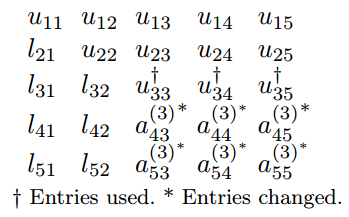
\includegraphics[width=0.49\linewidth]{png/rightlooking.png}
        \hfill
        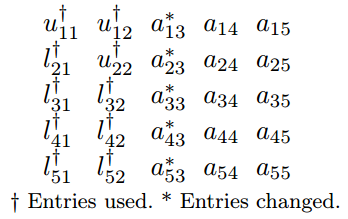
\includegraphics[width=0.49\linewidth]{png/leftlooking.png}
        \caption{Computational sequence for right- and 
        left-looking LU factorization.}
        \label{fig::rightleftlooking}
    \end{figure}

    While the left-looking is more efficient on modern hardware 
    than right-looking, it requires all the columns to the left 
    of the active column to be accessed while it is being 
    updated. Unless the matrix is small, these columns will not 
    fit into the cache, so that access can be slow.
\end{exm}

\subsection{Partial pivoting}
\begin{exm}
    The Gaussian elimination breaks down when $a_{kk}^{(k)}=0$, 
    illustrated by the case
    $$
        \begin{bmatrix}
            0&1\\2&3
        \end{bmatrix}
        \begin{bmatrix}
            x_1\\x_2
        \end{bmatrix}=
        \begin{bmatrix}
            4\\5
        \end{bmatrix}.
    $$ 
    Exchanging the first and second rows completely avoids 
    this difficulty. So at the $k$-th step of Gaussian 
    elimination where $a_{kk}^{(k)}=0$, we have to exchange 
    row $k$ with row $i$ satisfied $i>k$ and $a_{ik}^{(k)}
    \neq 0$. The only way this can break down is if 
    $$
        a_{kk}^{(k)}=a_{k+1,k}^{(k)}=\ldots=a_{nk}^{(k)}=0.
    $$ 
    In this case, $\mA$ is singular and the corresponding 
    equation does not have a unique solution.
\end{exm}

\begin{exm}
    \label{exm::instable}
    Assuming we are solving
    $$
        \begin{bmatrix}
            0.001&2.42\\1.00&1.58
        \end{bmatrix}
        \begin{bmatrix}
            x_1\\x_2
        \end{bmatrix}=
        \begin{bmatrix}
            5.20\\4.57
        \end{bmatrix}
    $$ 
    using a hypothetical computer with a 3-decimal 
    floating-point representation of the form 
    $\pm d_1.d_2d_3\times 10^i$ where $i$ is an integer, 
    $d_1,d_2,d_3$ are decimal digits and $d_1\neq 0$ unless 
    $d_1=d_2=d_3=0$. The triangular system that results from 
    applying Gaussian elimination is
    $$
        \begin{bmatrix}
            0.001&2.42\\0&-2420
        \end{bmatrix}
        \begin{bmatrix}
            x_1\\x_2
        \end{bmatrix}=
        \begin{bmatrix}
            5.20\\-5200
        \end{bmatrix}.
    $$ 
    The computed solution is 
    $$
        \tilde{\mathbf{x}}=\begin{bmatrix}
            \tilde{x}_1\\\tilde{x}_2
        \end{bmatrix}=
        \begin{bmatrix}
            0.00\\2.15
        \end{bmatrix},
    $$
    while the exact solution is
    $$
        \mathbf{x}=\begin{bmatrix}
            x_1\\x_2
        \end{bmatrix}\approx
        \begin{bmatrix}
            1.18\\2.15
        \end{bmatrix}.
    $$
    The error is not small compared with the exact solution.

    However, when we exchange the first and the second row, the 
    factorization will be
    $$
        \begin{bmatrix}
            1.00&1.58\\0.001&2.42
        \end{bmatrix}=
        \begin{bmatrix}
            1\\0.001&1
        \end{bmatrix}
        \begin{bmatrix}
            1.00&1.58\\&2.42
        \end{bmatrix},
    $$ 
    and the computed solution is 
    $$
    \tilde{\mathbf{x}}=\begin{bmatrix}
        \tilde{x}_1\\\tilde{x}_2
    \end{bmatrix}\approx
    \begin{bmatrix}
        1.17\\2.15
    \end{bmatrix},
    $$ 
    which is almost correct.
\end{exm}

\begin{defn}[Partial pivoting]
    One reason why we might get growth that destroys smaller 
    values in the course of the computation comes from having a 
    very large multiplier. A solution to this is to require 
    that the inequality $|l_{ij}|\leq 1$ should hold for the 
    coefficients of the matrix $\mL$. This can be achieved by 
    scanning the $k$-th column below the main diagonal to 
    determine its entry of largest magnitude, the row 
    containing this entry is exchanged with the $k$-th row, 
    therefore $|a_{kk}^{(k)}|\geq |a_{ik}^{(k)}|,\,i>k$ now.
    This strategy is called \textit{partial pivoting}.
\end{defn}

\begin{defn}[Full pivoting]
    At each step in Gaussian elimination, we can choose the 
    pivot to be the largest entry in the remaining submatrix 
    rather than only in the $k$-th row. 
    That is, row and column interchanges are performed at 
    each step to ensure that $|a_{kk}^{(k)}|\geq |a_{ij}^{(k)}|,
    \,i\geq k,j\geq k$ all hold. This strategy is called 
    \textit{full} or \textit{complete pivoting}.
\end{defn}

\begin{thm}
    \label{thm::fullpivot}
    By Gaussian elimination with full pivoting, any nonsingular 
    $\mathbb{R}^{n\times n}$ matrix can be factorized as 
    $\mP\mA\mQ=\mL\mU$, where $\mP$ and $\mQ$ are permutation 
    matrices, $\mL$ is unit lower triangular and  $\mU$ is 
    upper triangular.
\end{thm}
\begin{proof}
    Define elementary permutation matrix $\mI_{pq}$ as the 
    matrix obtained from $\mI$ by exchanging the $p$-th and 
    $q$-th columns (rows). $\mI_{pq}\mA$ exchanges the $p$-th 
    and $q$-th rows of $\mA$ and $\mA\mI_{pq}$ exchanges the 
    $p$-th and $q$-th columns of $\mA$.

    At each step of the full pivoting Gaussian elimination, the 
    row interchange and column interchange can be represented 
    as $\mP_k=\mI_{kp}$ and $\mQ_k=\mI_{kq}$, where $(p,q)$ is 
    the position of the largest entry. So the Gaussian 
    elimination can be represented by
    $$
        \mL_{n-1}\mP_{n-1}\ldots\mL_1\mP_1\mA\mQ_1\ldots\mQ_{n-1}=\mU.
    $$ 
    Define $\mQ=\mQ_1\ldots\mQ_{n-1},\,\mP=\mP_{n-1}\ldots\mP_1,\,
    \mL=\mP(\mL_{n-1}\mP_{n-1}\ldots\mL_1\mP_1)^{-1}$, then we have
    $$
        \mP\mA\mQ=\mL\mU.
    $$ 

    It is obvious that $\mP$ and $\mQ$ are permutation 
    matrices and $\mU$ is upper triangular, so we only need to 
    show $\mL$ is unit lower triangular. Actually $\mL=\mP_{n-1}
    \ldots\mP_2\mL_1^{-1}\mP_2\mL_2^{-1}\ldots\mP_{n-1}\mL_{n-1}^{-1}
    $ because $\mP_k\mP_k=I$. Define
    $$
        \mL^{(1)}=\mL_1^{-1},\,\mL^{(k)}=\mP_k\mL^{(k-1)}\mP_k
        \mL_k^{-1},\,k=2,\ldots,n-1,
    $$  
    then $\mL=\mL^{(n-1)}$. We can verify
    \begin{equation}
        \label{eq::fullpivL}
        \mL^{(k)}=
        \begin{bmatrix}
            \mL_{11}^{(k)}&0\\
            \mL_{21}^{(k)}&\mI_{n-1}
        \end{bmatrix},\,k=1,\ldots,n-1
    \end{equation}
    by induction, where $\mL_{11}^{(k)}$ is a unit lower 
    triangular matrix with entries norm no greater than $1$, 
    $\mL_{21}^{(k)}$ is a $\mathbb{R}^{(n-k)\times k}$ matrix 
    with entries norm no greater than $1$, $\mI_{n-1}$ is the 
    unitary matrix of order $(n-k)$.

    The induction base clearly holds for $k=1$ because of the 
    definition of $\mL^{(1)}=\mL_1^{-1}$. Now suppose that 
    \eqref{eq::fullpivL} holds for $k-1$. Then
    $$
        \mL^{(k)}=\mP_k\mL^{(k-1)}\mP_k\mL_k^{-1}=
        \begin{bmatrix}
            \mL_{11}^{(k-1)}&0\\
            \tilde{\mL}_{21}^{(k-1)}&\tilde{\mL}_k^{-1}
        \end{bmatrix},
    $$ 
    where $\tilde{\mL}_{21}^{(k-1)}$ is obtained from 
    $\mL_{21}^{(k-1)}$ by exchanging its first and $(p-k+1)$-th 
    rows, and
    $$
        \tilde{\mL}_k^{-1}=
        \begin{bmatrix}
            1\\
            l_{k+1,k}&1\\
            l_{k+2,k}&0&1\\
            \vdots&\vdots&\ddots&\ddots\\
            l_{nk}&0&\cdots&0&1
        \end{bmatrix}.
    $$ 
    So \eqref{eq::fullpivL} holds for $k$, which complete the 
    inductive proof.
\end{proof}

\begin{prop}
    Since partial pivoting can be viewed as a special case of 
    full pivoting, any nonsingular $\mathbb{R}^{n\times n}$ 
    matrix can be factorized as $\mP\mA=\mL\mU$, where $\mP$ 
    is a permutation matrix, $\mL$ is unit lower triangular and  $\mU$ is upper triangular.
\end{prop}

\begin{alg}
    By Theorem \ref{thm::fullpivot}, we can still use a single 
    two-dimensional array by writing $\mL$ in the lower 
    triangular part excluding the unit diagonal. The full 
    pivoting Gaussian elimination is then as follows.
    \IncMargin{1em}
    %\LinesNumbered
    \begin{algorithm}[H]
        \caption{Gaussian elimination with full pivoting}
        \SetKwInOut{Precond}{Preconditions}
        \SetKwInOut{Postcond}{Postconditions}

        \KwIn{$\mA\in\mathbb{R}^{n\times n}$}
        \KwOut{$\mathbf{u},\mathbf{v}\in\mathbb{Z}^{n-1}$}
        \Postcond{$\mL$ is stored in the lower triangular part 
        of $\mA$ excluding the unit diagonal, $\mU$ is stored 
        in the upper triangular part of $\mA$, $\mathbf{u}, 
        \mathbf{v}$ record $\mP, \mQ$ seprately}

        \BlankLine
        \For{$k=1,2,\ldots,n-1$}{
            Find $(p,q)$ s.t. $|\mA(p,q)|=\max\{|\mA(i,j)|:
            i=k:n,j=k:n\}$\;
            $\mA(k,1:n)\leftrightarrow \mA(p,1:n)$\;
            $\mA(1:n,k)\leftrightarrow \mA(1:n,q)$\;
            $u(k)=p,\,v(k)=q$\;
            \If{$\mA(k,k)==0$}{
                Full pivoting Gaussian elimination is failed
            }
            $\mA((k+1):n,k)=$ $\mA((k+1):n,k)/\mA(k,k)$\;
            $\mA((k+1):n,(k+1):n)=\mA((k+1):n,(k+1):n)-$ 
            $\mA((k+1):n,k)\mA(k,(k+1):n)$\;
        }
    \end{algorithm}
    \DecMargin{1em}
\end{alg}



\subsection{Block factorization}
\begin{alg}
    \label{exm::blockfactorize}
    In Example \ref{exm::leftlooking}, we show that when the 
    matrix is large, the columns in left-looking method will not 
    fill into the cache, the solution to this problem is to group 
    the updates by blocks. The most useful form is using the 
    left-looking algorithm until a given number $m$ of columns 
    has been factorized, then performing a right-looking block 
    update. If $m$ columns fit into cache, we can factorize the 
    first $m$ columns with one data movement.

    Let us partiation the matrix as
    $$
        \mA=
        \begin{bmatrix}
            \mA_{11}&\mA_{12}\\\mA_{21}&\mA_{22}
        \end{bmatrix},
    $$ 
    where $\mA_{11}$ is of order $m\times m$. Once the 
    processing of the first $m$ columns is complete, we will 
    have the factorization
    $$
        \begin{bmatrix}
            \mA_{11}\\\mA_{21}
        \end{bmatrix}=
        \begin{bmatrix}
            \mL_{11}\\\mL_{21}&\mI
        \end{bmatrix}
        \begin{bmatrix}
            \mU_{11}\\0
        \end{bmatrix}.
    $$ 
    If we had updated the remaining columns, the factorization 
    would have been
    $$
        \begin{bmatrix}
            \mA_{11}&\mA_{12}\\\mA_{21}&\mA_{22}
        \end{bmatrix}=
        \begin{bmatrix}
            \mL_{11}\\\mL_{21}&\mI
        \end{bmatrix}
        \begin{bmatrix}
            \mU_{11}&\mU_{12}\\&\ddot{\mA}_{22}
        \end{bmatrix}.
    $$ 
    By equating corresponding blocks we find the relations
    $$
        \mL_{11}\mU_{12}=\mA_{12},\,\ddot{\mA}_{22}=\mA_{22}-\mL_{21}\mU_{12},
    $$
    $\ddot{\mA}_{22}$ is known as the \textit{Schur complement} 
    of $\mA_{11}$. 

    The columns of $\mU_{12}$ may be found by forward 
    substitution through $\mL_{11}$. The remaining for the 
    given matrix are exactly those that would be made for 
    factorizing the matrix $\ddot{\mA}_{22}$, this can be done 
    by the same strategy.
\end{alg}

\begin{exm}[Implicit block factorization]
    In normal block factorization in Example 
    \ref{exm::blockfactorize}, we calculate 
    \begin{align*}
        &\mA_{11}=\mL_{11}\mU_{11},\\
        &\mL_{11}\mU_{12}=\mA_{12},\\
        &\mL_{21}\mU_{11}=\mA_{21},\\
        &\ddot{\mA}_{22}=\mA_{22}-\mL_{21}\mU_{12}=\mL_{22}
        \mU_{22}.
    \end{align*}
    An interesting variation, known as \textit{implicit block 
    facotrization}, results if the factorization $\mA_{11}=
    \mL_{11}\mU_{11}$ and $\ddot{\mA}_{22}=\mL_{22}\mU_{22}$ 
    are stored, but $\mU_{12}$ is not. When $\mU_{12}$ is 
    needed as a multiplier, $\mL_{11}^{-1}\mA_{12}$ is used 
    instead. This has little merit in the dense case, but in 
    the sparse case it is extremely like that $\mU_{12}$ has 
    many more entries than $\mA_{12}$ so less storage will be 
    needed and sometimes less computation also.
\end{exm}

